\RequirePackage[T1]{fontenc}
\documentclass[conference]{IEEEtran}
\IEEEoverridecommandlockouts
\usepackage{mathptmx}
\usepackage{cite}
\usepackage{amsmath,amssymb}
\usepackage{graphicx,booktabs,array}
\usepackage{xcolor}
\usepackage[hyphens]{url}
\usepackage{tikz}
\usetikzlibrary{arrows.meta,positioning,fit}
\usepackage{pgfplots}
\pgfplotsset{compat=1.18}
\usepackage[hidelinks,pdfauthor={},pdftitle={Beyond Bandwidth: Transaction-Aware Design of Ethernet Scale-Up Fabrics for AI Inference}]{hyperref}
\newcommand{\sys}{the transaction-aware simulator}
\newcommand{\us}{\ensuremath{\mu\mathrm{s}}}
\begin{document}
\pagenumbering{arabic}
\title{Beyond Bandwidth: Transaction-Aware Design of Ethernet Scale-Up Fabrics for AI Inference}
\author{\normalsize Working Draft --- ISCA 2026 Template --- Not Submitted}
\maketitle
\thispagestyle{plain}\pagestyle{plain}

\begin{abstract}
Ethernet scale-up fabrics increasingly motivate joint design of accelerator I/O, switching, and remote memory. Provisioning such systems by aggregate bandwidth alone obscures the cost of forming transactions, reserving credits, and sustaining memory-level concurrency. We develop a transaction-aware simulation methodology that couples task dependencies, AXI-like records, packet aggregation, SUE forwarding and credit flow control, and shared accelerator and remote-memory resources. The model also includes a transactional PCIe reference path with finite tags, credits, and shared host memory. Preliminary, reproducible experiments expose two pitfalls. In a mixed-traffic inference window, best-effort aggregation reduces switched data-frame count by more than 92\%, but reduces completion time by only 6.43--9.33\% across three routing seeds. In a separate four-way precision/scheduler experiment, refining time resolution from 1\,ns to 1\,ps reduces a PCIe-backed representative block from 372.474 to 289.155\,\us; polling versus event notification does not change the result at either precision. We trace the latter effect to quantized service budgets, including inflated per-packet link occupation. These observations motivate a transaction-aware design space for aggregation, credit allocation, and memory admission. This working draft reports implemented mechanisms and preliminary simulation evidence; a joint control policy, finite switch packet-rate modeling, and hardware calibration remain future evaluation work.
\end{abstract}

\section{Introduction}
Scale-up systems must move more than bulk collective traffic. A mixture-of-experts (MoE) layer exchanges token activations among expert owners; a key--value (KV) access moves attention state; a fine-grained lookup may issue many small remote reads. Even when their byte volumes fit within nominal link bandwidth, these operations can require very different numbers of requests, responses, and occupied queue entries. Their completion times determine when dependent computation can proceed.

This distinction becomes important in systems that attach memory processing units (MPUs) to the same fabric as accelerators. An MPU adds capacity and memory service bandwidth, but consuming that bandwidth requires sufficient request concurrency and a return path that can drain completed data. The accelerator must then write and consume the data through finite local memory resources. Host memory accessed through PCIe offers another path, with its own DMA admission, tags, shared links, and DDR contention. A fair comparison must represent both paths at compatible levels of detail.

Existing frameworks establish important foundations. ASTRA-sim 2.0 supports graph-based parallel workloads, heterogeneous hierarchical networks, and disaggregated memory modeling~\cite{astra2}. SimAI connects training-framework, kernel, collective, and network behavior~\cite{simai}. CXL-DMSim emphasizes full-system memory expansion with silicon validation~\cite{cxldmsim}. Our objective is complementary: expose how transaction formation and resource admission interact within an Ethernet scale-up inference window. We do not claim that configurable topology, task graphs, or remote-memory simulation are new in isolation.

Our central thesis is that architecture decisions require a vector of resource demands rather than a single byte count. Two workloads with equal useful bytes can occupy different packet-processing opportunities, credit windows, and memory slots. Conversely, an optimization that reduces packets may not reduce the critical path proportionally. A model that accidentally rounds away these distinctions can even reverse a design comparison.

This draft makes three bounded contributions. First, it describes an implemented task-to-transaction-to-packet model with explicit resource and completion boundaries. Second, it presents measured packet-aggregation and time-precision case studies, with frozen inputs and accounting checks. Third, it formulates a design and validation agenda for aggregation and credit allocation under fixed hardware budgets. The proposed joint policy is not implemented or evaluated in the present results. The reported windows are representative inference blocks, not full-model token latency or throughput.

\section{Design Problem and Scope}
\subsection{A heterogeneous scale-up node}
We study accelerators containing four compute Dies, each with eight external ports and a bidirectional on-package ring. TP denotes tensor parallelism; DP denotes replication of public-layer parameters and requests; EP distributes experts. TP and EP describe different phases over the same Dies and must not be multiplied to infer hardware count. In our 16-chip cases, TP4 groups remain within a chip, public computation has DP16, and global EP64 places experts across all 64 Dies.

Eight independent Ethernet rails connect one port per Die and one port per MPU to each rail switch. For 16 chips and two MPUs, a switch uses $16\cdot4+2=66$ ports. This experimental topology is not the two-switch pure-XPU16 topology. An MPU is a modeled memory service endpoint, not a GPU running kernels. Its nominal memory bandwidth does not imply that every requester receives that rate.

The compute model reserves a per-Die FIFO service resource based on work and effective compute rate. HBM service uses configurable capped max--min sharing among traffic classes. These abstractions preserve contention and dependencies but do not execute GPU instructions, caches, DRAM banks, or complete attention kernels. Architectural results must be interpreted at that abstraction level.

\subsection{The design variables}
The relevant choices include packet aggregation eligibility and urgency, VC mapping and credit partitioning, memory request concurrency, and placement between HBM, remote memory, and host DDR. The objective is to minimize completion time under fixed capacity, buffer, and credit budgets. Fair comparisons cannot give an optimized policy more aggregate buffering or omit the costs of its request path.

A small request can be causally important despite contributing few bytes: delaying it prevents its response from being generated. Conversely, a large response may dominate both bandwidth and credit occupancy. Byte-proportional credit allocation is therefore a baseline to test, not a theorem. We study these questions without asserting that arbitrary separation of request and response channels is protocol-safe.

\section{Transaction-Aware Modeling}
Figure~\ref{fig:architecture} summarizes the modeled layers and the alternative host-memory path.
\begin{figure*}[t]
\centering
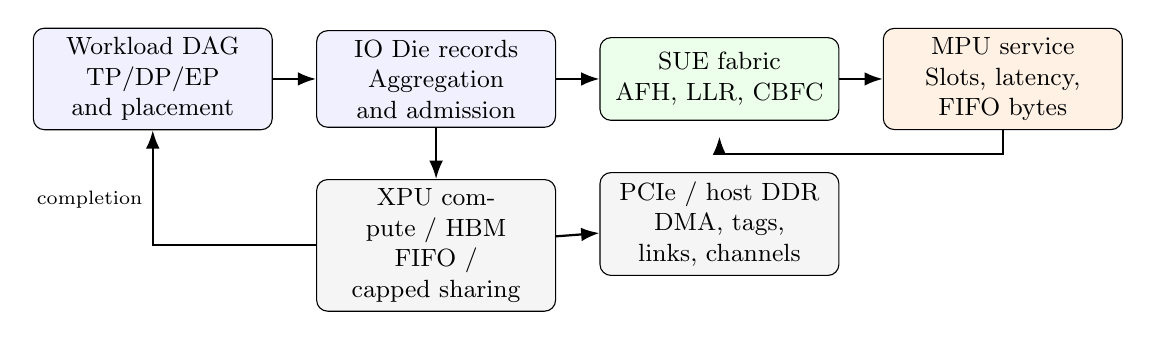
\begin{tikzpicture}[font=\small, box/.style={draw,rounded corners,align=center,minimum height=1.05cm,text width=2.8cm},arr/.style={-{Latex},thick}]
\node[box,fill=blue!6] (dag) {Workload DAG\\TP/DP/EP and placement};
\node[box,fill=blue!6,right=0.55cm of dag] (io) {IO Die records\\Aggregation and admission};
\node[box,fill=green!8,right=0.55cm of io] (net) {SUE fabric\\AFH, LLR, CBFC};
\node[box,fill=orange!10,right=0.55cm of net] (mpu) {MPU service\\Slots, latency, FIFO bytes};
\node[box,fill=gray!8,below=0.65cm of io] (hbm) {XPU compute / HBM\\FIFO / capped sharing};
\node[box,fill=gray!8,below=0.65cm of net] (pcie) {PCIe / host DDR\\DMA, tags, links, channels};
\draw[arr] (dag)--(io);\draw[arr] (io)--(net);\draw[arr] (net)--(mpu);
\draw[arr] (mpu.south) -- ++(0,-0.3) -| ([yshift=-0.2cm]net.south);
\draw[arr] (io)--(hbm);\draw[arr] (hbm)--(pcie);
\draw[arr] (hbm.west)-|node[pos=0.7,left,font=\scriptsize]{completion}(dag.south);
\end{tikzpicture}
\caption{Implemented modeling layers. Return traffic follows the modeled fabric and original port; the drawing summarizes logical dependencies, not physical wiring. PCIe is an alternative host-memory path. Finite response staging at MPU completion is a known missing backpressure boundary.}
\label{fig:architecture}
\end{figure*}

\subsection{Workload and completion semantics}
A task graph defines computation, local data movement, and network operations. Ordinary dependency edges wait for transaction completion, including acknowledgement return where applicable. Receive-dependency edges can release a consumer when the destination has received the required data, allowing acknowledgement transmission to overlap with subsequent work. A configurable notification delay follows the corresponding completion event.

MoE communication uses feature striping across the ranks of an active TP group. An expert waits for its required input slices and executes once. Output slices return to the participating ranks; local reduction and TP exchange reconstruct the public representation. The workload generator does not gather all traffic at the first TP rank. Its token-to-expert choices remain synthetic rather than measured execution traces. Our frozen workloads include a temporal expert-reuse assumption, which must be swept or replaced with traces before making deployment-wide claims.

\subsection{AXI-like record formation and aggregation}
Endpoints represent traffic using AW, W, B, AR, and R records. W and R have 256-byte data granularity; AW and W belonging to one request remain together. Compatible records may share a packet only when they use the same output port, destination identifier, VC, and transaction class. AR aggregates with AR, B with B, R with R, and AW+W units with other AW+W units.

The implemented best-effort policy merges eligible records already available to the packetizer, subject to packet-size and queue constraints. It does not introduce an intentional waiting timer solely to fill a packet. An isolated eligible record can therefore depart without waiting for hypothetical future traffic. The no-packing baseline retains the same transaction decomposition and disables cross-request aggregation.

This layer models record sizes, identity, matching, and timing. It is not a complete AXI conformance model: real AXI ID reuse, memory consistency, atomic operations, and all address-boundary requirements are outside its scope. Fine-grained gather traffic is generated from task-level byte counts rather than a captured physical-address stream.

\subsection{Fabric and flow control}
The simulator uses the existing SUE AFH forwarding, LLR retry, and CBFC implementation. Ports have independent VC state; a VC is not a Die or a physical rail. Static forwarding respects the configured routing domains. Topologies that require destination-side Die transfer use the finite-resource local ring and the configured return-port semantics.

We distinguish useful bytes, data-frame wire bytes, and protocol-control activity. The packing experiment counts each data frame once at switch egress, avoiding double counting across its two physical links. The current wire convention includes modeled headers, minimum padding, and preamble, but does not add a separate FCS beyond the implemented layout. IFG is not counted as wire bytes. These conventions are necessary when converting counters into packet rates or occupancy.

The current switch does not have an independently calibrated finite packet-processing-rate limit. Consequently, observed Mpps describes offered or carried load, not a validated switch-capacity requirement. An idle-to-nonempty scheduling path can also bypass a pending IFG timer. We report this limitation rather than interpreting the present traces as strict Ethernet line-rate validation.

\subsection{Memory admission and local consumption}
An MPU accepts individual 256-byte memory transactions into a finite in-flight window. After admission, a configurable access latency can overlap across requests. Ready transactions share one FIFO byte-service budget per MPU. At 190\,GB/s, each 1\,ns service window supplies 190 bytes, and unused bytes within that window can serve the next ready transaction. Slots are released at memory-service completion.

The present implementation permits queued requests awaiting memory admission and releases slots before a completed response has fully drained into the network. It therefore lacks a complete finite-buffer chain from response staging back to MPU admission. This omission is particularly relevant to future credit-allocation studies and must be corrected before claiming bounded-buffer guarantees under overload.

XPU HBM sharing is defined by traffic class rather than by individual request. A source constrained by an external interface consumes at most its cap; other active classes can use the remaining bandwidth. This avoids rewarding a source for splitting work into more requests. Some SUE-to-HBM paths still stage a complete message before modeled HBM service, rather than providing packet-by-packet storage-credit coupling.

\subsection{Transactional PCIe reference path}
The host-memory alternative includes per-chip DMA engines, descriptor admission, tags, in-flight byte limits, request and Completion segmentation, and finite credit and receive resources. Four chips share a modeled NUMA-side uplink; eight chips form a two-socket host. DDR traffic competes across channel resources after a fixed access delay. The destination HBM write completes before its receive-buffer space is released.

This is a transaction-level service model, not a PCIe PHY, FLIT, or replay implementation. Configured link rates describe serialization budgets including the model's packet overhead. The same model and workload must be used for a PCIe-only baseline and any hybrid comparison; otherwise an apparent memory-pool benefit may come from a mismatched reference path.

\subsection{Transaction state and resource ownership}
A transaction-aware model must specify where a request resides while it is blocked. Merely delaying its completion is insufficient: the outstanding work may occupy an endpoint queue, a link credit, a memory slot, or none of these resources. We distinguish a producer-owned request that has not been admitted from an admitted record that consumes a modeled hardware queue entry. A failed admission leaves the former with its producer. Registering a wakeup callback does not itself allocate another hardware slot.

The implemented read path decomposes an operation into AR generation, fabric delivery, memory admission, overlapping access latency, bandwidth service, R generation, return transport, and destination consumption. Memory admission and response generation are distinct events. The read's useful-byte count belongs to returned data, not to the AR descriptor; adding both would double-count the logical payload. A network write instead carries an indivisible AW+W record and later generates a B response. A MoE combine is another write operation rather than the B acknowledgement for dispatch. This distinction matters when attributing response traffic to the application.

For a request $j$, let $a_j$ be arrival at the MPU, $m_j$ admission, $r_j$ latency readiness, $s_j$ first bandwidth service, and $e_j$ memory completion. The implemented service obeys
\begin{equation}
 a_j\leq m_j,\quad r_j=m_j+L_j,\quad s_j\geq r_j,\quad e_j\geq s_j.
\end{equation}
Admission waiting is $m_j-a_j$; latency waiting is $r_j-m_j$; bandwidth waiting is $s_j-r_j$. These intervals describe one request. Their sums over requests measure accumulated pressure, not an end-to-end application latency. Response transport and HBM service occur after or alongside other requests' intervals and require separate accounting.

This decomposition also exposes a limitation of the present model. At $e_j$, the memory slot is released even if the generated R record cannot immediately enter its output queue. The completed response remains pending in the adapter. Thus a memory-slot bound currently constrains memory service, not the entire request-to-response round trip. Applying a full network RTT to that slot bound would overstate its modeled restriction. Conversely, claiming a fully bounded memory subsystem would overlook pending response storage. A complete implementation must separately budget memory slots and completed-response bytes.

\subsection{Packetizer eligibility and ordering}
The packetizer operates on a per-output-port record queue. Its first queued record determines the packet's compatibility class. It scans queued records and selects eligible records of that class until the configured packet capacity is reached. Records of other classes can remain queued while compatible later records are selected. Selection therefore preserves an eligibility rule rather than a global FIFO over every transaction class. Evaluating a different selection rule requires an explicit policy change; it should not be hidden inside a purportedly equivalent implementation optimization.

The compatibility key includes source Die and port, destination chip and Die, destination proxy where applicable, VC, and record kind. This is stricter than equal destination chip alone. Two records sent toward different destination Dies or through different forwarding proxies cannot be merged merely because the same chip eventually owns the data. AW and W are represented as one eligible unit, preventing aggregation from separating a write address from its associated data. Each response retains its relation to the originating transaction even when several responses share one fabric packet.

After packet formation, the endpoint checks whether its device egress can admit the packet. If not, it leaves the selected records in their queue. On successful admission, it removes those records and reserves the next packet-formation opportunity using the modeled endpoint wire-slot duration, rounded to the configured whole-nanosecond opportunity schedule. The fabric can add further delay through arbitration, control traffic, and credit availability. Consequently, packetizer opportunities and actual link transmissions are different timestamps. The precision experiment does not imply that every endpoint scheduling boundary was converted into a fractional-nanosecond issue mechanism.

Best-effort packing is sensitive to simultaneous arrivals. A queue that has accumulated compatible records during backpressure can form a large packet without an explicit batching delay. Under light load, the same policy may send much smaller packets. The resulting packet-size distribution is an output of workload timing and contention, not a fixed user-provided average. Comparing policies using only a mean packet size would miss this feedback.

\subsection{A bounded completion path as a design extension}
Before evaluating aggressive credit allocation, we propose adding a finite completion-store resource at each MPU. A memory operation would need either a reserved response slot before service or available response bytes at completion. The design must choose and document one of these semantics. Early reservation prevents completion-stage overflow but can hold space throughout the access latency. Late reservation increases overlap but requires a place to retain an otherwise completed operation while waiting for storage.

Neither rule should silently increase physical capacity. The state machine must account for requests awaiting admission, in-service data, completed responses, and endpoint records without charging the same storage twice. If response storage is full, the corresponding backpressure should prevent an unbounded stream of newly admitted operations. This extension could use an explicit admission condition combining memory-slot availability and response-space reservation. It is not part of the reported experiments, so its impact on throughput or fairness remains unknown.

Correctness checks should verify conservation at every state transition: generated requests equal pending plus active plus completed requests; delivered useful bytes equal the sum of completed data fragments; and memory and response occupancy never exceed their independent limits. A final zero-pending check detects stuck operations but is insufficient on its own: a simulation can finish while having exceeded a buffer transiently. Peak and time-series assertions are therefore required as well.


\section{Event Scheduling and Numerical Fidelity}
\subsection{Notification replaces failed admission attempts}
Periodic polling can make simulator execution cost depend on how long an unavailable resource remains unavailable. If $K$ blocked producers each retry every $\Delta$ time units for duration $T$, their failed checks can scale approximately as $KT/\Delta$. These checks do not transfer useful data. An event-driven adapter instead registers waiting producers and schedules a retry when a relevant resource changes state. This reduces simulator work, but it must preserve the resource constraints rather than granting capacity on notification.

The current IO adapter keeps waiting producers associated with their original retry-clock phase. When queue space becomes available, it computes the next eligible retry time for a waiting phase and arms a port-level event. Within that phase, registered producers are resumed in registration order while space remains. Device egress blockage uses a release notification from the endpoint device. A notification is an opportunity to retry admission, not proof that a complete packet can be transmitted without checking egress and credit state.

This scheduling change does not alter AFH forwarding or the LLR/CBFC protocol algorithms. It can nevertheless change the order in which simultaneous callbacks enter an adapter queue. Since packet formation depends on which compatible records are present at that instant, different event insertion orders can change packet sizes and individual task times. We therefore distinguish protocol invariance, resource-contract invariance, and trace equivalence. The first two do not establish the third.

For an optimization claimed to preserve a particular experiment, we compare its input hashes, total useful bytes, completion status, and timing records. If traces differ, we report the difference instead of treating delivery alone as proof of timing equivalence. The PCIe case in this paper passes a stronger paired check: four families of output files match exactly between wakeup modes at each precision. That observation is deliberately scoped to the paired workload and cannot be generalized to all queue-contention patterns.

\subsection{Clock resolution is not hardware issue frequency}
A discrete-event simulator advances to scheduled events rather than executing one iteration for every time quantum. Moving from 1\,ns to 1\,ps resolution therefore does not imply one thousand times as many event callbacks. The event count depends on modeled operations and scheduling decisions. A 200\,ns memory access remains a delayed event; a 1\,ns admission interval remains a 1\,ns interval. Finer timestamps allow the model to represent service and propagation durations between those boundaries.

There are at least three timing contracts: event timestamp representation, resource-service granularity, and producer issue frequency. The current configuration separates them. Global time is represented in picoseconds. MPU bandwidth service proceeds in 1\,ns windows with a byte budget. IO producers retain their configured request intervals, and packet formation has its own opportunity schedule. A future cycle-accurate IO model would additionally constrain how many operations a particular hardware block can accept each cycle; timestamp precision alone supplies no such constraint.

When a byte server has a fixed cycle, it should conserve residual capacity within the cycle. Serving a 256-byte transaction on a 190-byte-per-cycle server requires at least two service windows for that transaction, but the second window need not be dedicated exclusively to its remaining 66 bytes. The next ready FIFO transaction may consume the remaining 124 bytes. Rounding every transaction to two exclusive cycles would create a different and lower-bandwidth server. The same principle explains why coarse per-packet serialization can distort the PCIe reference path.

\subsection{Invariants and reproducibility boundaries}
We use three classes of checks. Structural checks reject invalid dependency edges, illegal endpoint identities, and inconsistent compiled inputs. Conservation checks compare generated, transmitted, received, and resource-serviced bytes while distinguishing logical data from protocol overhead. Temporal checks verify that a consumer starts only after its declared completion condition and that resource occupancy and service order match the selected model.

These checks establish internal consistency; none substitutes for external validation. A precisely reproducible model can be consistently wrong about a switch pipeline or an IO Die. Conversely, measurements can reveal the correct throughput while leaving insufficient evidence to explain queue occupancy. We retain both functional invariants and a separate calibration requirement so that a successful regression is not mislabeled as silicon accuracy.

An experiment records resolved inputs, component hashes, the simulator binary identity, status, and raw statistics. Multiple conditions execute as independent processes; this is different from parallelizing one simulated timeline. Capacity-rejected conditions are reported as such, without assigning a completion time. Timeouts and unfinished graphs remain failures rather than disappearing from an average. The harness facilitates these practices, but its presence is not itself evidence for the scientific claims.


\section{Resource Bounds and Design Hypotheses}
A useful first diagnostic for one traffic class is
\begin{equation}
 B_{\mathrm{useful}}\leq\min\left(B_l\eta,\;P_s\bar u,\;\frac{W_c\eta}{T_c},\;\frac{N_m q}{T_m},\;B_m\right),
\label{eq:bound}
\end{equation}
where $B_l$ is link byte rate, $\eta$ useful-to-wire efficiency, $P_s$ packet service rate, $\bar u$ useful bytes per packet, $W_c$ the credit window in wire-equivalent bytes, $T_c$ its holding time, $N_m$ memory slots, $q$ useful bytes per admitted transaction, and $T_m$ slot residence. The bound assumes a consistent accounting interval and charging convention. It is not a replacement for dependency or shared-resource simulation; different classes and paths compete for these quantities.

For example, 128 memory slots, 256 bytes per slot, and at least 200\,ns residence give an optimistic concurrency ceiling of 163.84\,GB/s, below a nominal 190\,GB/s memory server. Service and queueing can tighten that ceiling. This calculation explains why adding nominal memory bandwidth alone need not help. It is a bound, not a new measured throughput point.

Aggregation increases $\bar u$ and can improve $\eta$, but may change waiting and credit residence. A proposed packet-rate-limited switch would separate fixed pipeline latency from service initiation interval, with explicit parallel lanes and arbitration. Simply adding a fixed delay to each packet does not model a throughput ceiling. Similarly, per-message injection intervals are not a measured aggregate IO Die issue rate.

We propose investigating a bounded-delay aggregation and static credit-allocation policy. An offline search would choose legal per-class aggregation thresholds and credit partitions under fixed total credits and buffering. Runtime packetization would preserve destination, port, VC, and ordering rules and bound intentional waiting. Initial baselines would include no packing, current best-effort packing, fixed-delay packing, uniform credit partitioning, and byte-proportional partitioning. This policy remains a research proposal; this draft reports no benefit for it.

\subsection{From aggregate bandwidth to bottleneck regimes}
Equation~\ref{eq:bound} provides a way to organize experiments before performing a large design-space search. Its terms correspond to different regimes. A link-limited regime requires enough transactions and memory service to keep the physical path busy. A packet-limited regime instead exhausts packet-processing opportunities before reaching the link's byte budget. A credit-limited regime cannot sustain enough outstanding wire bytes over the credit holding time. A memory-concurrency regime cannot keep the server supplied despite adequate nominal bandwidth. The regimes can overlap, and their boundaries move as queueing changes holding times.

One useful dimensionless indicator is
\begin{equation}
 \chi_p=\frac{B_l\eta}{P_s\bar u}.
\end{equation}
If $\chi_p>1$, the packet service term is tighter than the link-bandwidth term under the stated traffic mix. This is a diagnostic rather than an independent prediction: $\eta$ and $\bar u$ can themselves depend on packing and load. Increasing link speed alone raises the numerator and can leave packet service as the limiting resource. Increasing aggregation can raise useful bytes per packet, but the measured timing cost of doing so must also enter the graph.

A corresponding memory-concurrency indicator is
\begin{equation}
 \chi_m=\frac{B_m T_m}{N_m q}.
\end{equation}
Values greater than one indicate that the chosen slot count cannot sustain the nominal memory bandwidth under the assumed residence time. For the optimistic 200\,ns residence and our 256-byte request size, sustaining 190\,GB/s requires at least
\begin{equation}
 N_m\geq\left\lceil\frac{190\times10^9\cdot200\times10^{-9}}{256}\right\rceil=149.
\end{equation}
This is only a necessary concurrency condition. Actual residence includes bandwidth service and possibly waiting, and a future design that retains slots through response staging would require a different bound. Setting the slot count to 149 would not guarantee 190\,GB/s in the simulator or hardware.

Credit provisioning has an analogous bandwidth-delay requirement, but its delay must match the actual release event. If a destination returns credits after accepting data into finite storage, downstream storage contention can increase credit residence even while propagation delay is fixed. Replacing that residence with bare link latency makes the credit bound artificially optimistic. A sweep should therefore record both the configured credit quantity and the measured distribution of holding times. This separates an undersized window from a downstream receiver that has stopped draining.

\subsection{Placement and path selection under shared resources}
A nominal-bandwidth placement rule might assign a fraction $f$ of remote bytes to MPU and the rest to PCIe. For a batch of $D$ independent bytes and two paths with constant effective rates $b_M$ and $b_P$, an idealized completion model is
\begin{equation}
 T(f)\approx\max\left(L_M+\frac{fD}{b_M},\;L_P+\frac{(1-f)D}{b_P}\right).
\end{equation}
Ignoring unequal startup latencies gives $f=b_M/(b_M+b_P)$. This familiar balancing argument is useful only if effective rates are known and the paths are sufficiently independent. Plugging in nominal aggregate memory and link bandwidths assumes the very issue the transaction model is intended to test.

In our target system, both paths eventually write and consume data through the same destination HBM. Their rates can depend on the fraction assigned to them, because more simultaneous returns change receive-buffer pressure and local service shares. MPU access also consumes SUE packet and credit resources shared with MoE communication. Increasing $f$ can therefore delay a critical MoE dependency even if it shortens the MPU portion of a bulk memory operation. The simple maximum of two independent transfer times omits this interference.

Chunk placement introduces a further distinction between a nominal fraction and a realized transaction assignment. A 256\,KiB chunking rule produces discrete work units, and the number assigned to a destination can change abruptly with node count. Equal total bytes do not imply equal arrival times or equal service demand at each Die. To diagnose a nonmonotonic placement curve, we would first inspect realized per-destination byte counts, packet counts, and request readiness, then use fixed-mapping and fixed-fraction controls. Without those controls, attributing every turning point to network congestion would be premature.

\subsection{Capacity benefit and latency benefit are different objectives}
An MPU can be useful even when a particular remote read is slower than a PCIe or local-HBM read, because it may change the amount of state the system can retain. That benefit requires a capacity-constrained evaluation. If the entire workload fits comfortably in local HBM, comparing remote reads against local reads primarily measures an access penalty, not the value of expanded capacity. Conversely, a capacity calculation alone cannot establish that additional requests can be served at a useful rate.

A fair capacity study should specify a fixed resource budget and an admission objective. Examples include the maximum number of requests whose state fits while meeting a latency target, or completion time at a fixed number of chips and equal available host memory. The model must account for which state is replicated, sharded, or cached. Counting a shared remote table once while duplicating the comparator unnecessarily would bias the result. Likewise, assigning every requester the full MPU bandwidth would mistake shared capacity for private service.

These distinctions suggest three separate outputs: admitted workload capacity, simulated service performance for admitted requests, and hardware-resource cost assumptions. They should not be collapsed into an unqualified acceleration claim. The preliminary experiments in this paper provide performance windows and resource observations; they do not establish a cost optimum or a serving-capacity improvement. The analytical regimes above identify which additional measurements would be needed to connect those objectives.


\section{A Transaction-Aware Design Proposal}
\subsection{Objective and fixed-budget constraints}
The observations motivate a specific research design: choose legal aggregation and credit configurations to shorten dependency-critical transactions while sustaining bulk traffic. We formulate the first version as an offline configuration problem rather than claiming an implemented adaptive controller. For traffic classes $k\in\mathcal K$, the variables are a maximum intentional aggregation wait $\tau_k$, a packet-size cap $p_k$, and a legal credit allocation $c_k$. The existing best-effort scheme is a no-intentional-wait baseline, not an oracle.

The search should obey
\begin{equation}
 \sum_{k\in\mathcal K}c_k=C_{\mathrm{total}},\qquad
 0\leq\tau_k\leq\tau_{\max},\qquad
 p_k\leq p_{\max},
\end{equation}
and an independently enforced total storage budget. Credits may refer to space at a different interface than the packetizer's record queue; equating them without a layout model would double-count or omit SRAM. Candidate designs must satisfy the protocol's minimum progress conditions, not only the sum constraint. The appropriate minima require a dependency analysis of the selected mapping.

The optimization objective should be completion time of the relevant application graph, with tail latency and starvation constraints, rather than packet count alone. A policy that reduces the mean frame count but indefinitely delays sparse lookup responses is not acceptable. Conversely, prioritizing every short packet can starve bulk KV returns and postpone computation waiting on those returns. We therefore treat both throughput and the age of dependency-blocking work as observables, while postponing any claim that a particular priority function is optimal.

\subsection{Candidate decision rules}
A practical first experiment would use a small, explicit candidate set. Packet caps could take several legal values; intentional waits could include zero and a few short intervals; credit partitions could be uniform, proportional to measured bytes, or selected by constrained search. The search would use training workloads only. A held-out set would vary arrival pattern, batch, context, destination skew, and locality to test whether the chosen configuration generalizes.

The runtime packetizer would enforce the same compatibility key as the baseline. A record becomes eligible for forced departure when its age reaches the class limit, while compatible queued records may be included up to the cap. The controller must avoid waiting for records that cannot legally share a packet. For example, spreading requests across more destinations can reduce aggregation opportunities even if the total offered byte rate is unchanged. A fixed waiting interval that is beneficial for a hot destination may only add latency for a sparse destination.

Credit allocations should initially remain static during a run. Dynamically transferring credits introduces additional protocol questions: how to avoid allocating the same buffer twice, how to reclaim credits already in flight, and how to prevent a class from losing all progress resources. These mechanisms are absent from the current implementation. Starting with static legal configurations isolates the value of better provisioning from the complexity and transient risks of online reallocation.

An implementation of this proposal would require instrumentation at policy decision points: oldest eligible record age, available packetizer space, in-use credits, class-specific service, and the downstream condition blocking progress. Recording only the chosen action would make it difficult to distinguish a mistaken decision from an inaccurate resource model. A policy trace should therefore include both action and observed state, while avoiding oracle access to future arrivals.

\subsection{Baselines, ablations, and fairness}
The principal baselines should include the current no-packing and best-effort modes, fixed waiting with uniform credits, best-effort packing with byte-proportional credits, and the proposed joint selection. A packing-only search and a credit-only search would identify whether the variables interact. Giving the joint design a larger maximum packet or a larger total credit budget than its competitors would confound the comparison; either hold these limits fixed or explicitly study the extra hardware cost.

Workloads used to select a configuration should not also determine the headline evaluation result. For example, one could select a static configuration using moderate batch and balanced routing, then evaluate it under low batch, high batch, skewed destinations, and changes in memory-slot availability. Report regressions as well as improvements. A robust design may trade a smaller median gain for fewer severe tail regressions; a single best point cannot demonstrate that property.

For replicated traffic sources, fairness must be defined at the level of independent service demand. Splitting one logical source into many simulator tasks should not increase its resource weight. Our current HBM model uses traffic classes for this reason. A packet policy must similarly distinguish the application's parallelism from an artificial increase in task count. Testing equivalent byte streams with different task decomposition is a useful adversarial check on the proposed mechanism.

\subsection{Progress and boundedness requirements}
A credit system can stall without losing data, and a simulation can appear to run forever while repeatedly checking a blocked queue. The proposed mechanism therefore requires more than final delivery in uncongested cases. For a bounded offered workload, every admitted transaction should eventually finish under stated assumptions about the fabric and memory server. Every finite buffer should remain within its limit throughout execution. At least one progress path must remain available when bulk responses consume most storage.

A proof of deadlock freedom is not provided in this draft. Before making such a claim, the design must construct its channel/resource dependency graph, including request admission, response storage, fabric credits, and local consumption. A stress test is useful but cannot replace that argument. Progress checks should also cover sparse traffic, mixed reads and writes, simultaneous completions, and a response queue that remains full for multiple service intervals.

This proposal deliberately avoids attributing measured improvements to an unimplemented mechanism. Its purpose is to define a falsifiable next step: if a fixed-budget joint configuration cannot outperform appropriately tuned independent baselines across held-out regimes, then the evidence would favor simpler provisioning. The present simulator and measurements provide the means to test that outcome rather than predetermine it.


\section{Experimental Methodology}
\begin{table}[t]
\centering\caption{Implemented configuration used for the reported cases.}
\label{tab:setup}
\small
\begin{tabular}{p{0.30\columnwidth}p{0.60\columnwidth}}
\toprule
Component & Configuration / scope\\\midrule
Accelerators & 16 chips, 4 Dies/chip; TP4, DP16, EP64\\
External ports & 8 ports/Die; 200\,Gb/s per port\\
MPU & 190\,GB/s one-way; 128 slots; 200\,ns latency\\
HBM & 1.875\,TB/s effective per Die; capped sharing\\
PCIe & 128\,GB/s per chip; 512\,GB/s shared uplink per 4 chips\\
Host DDR & 2 sockets/host, 12 channels/socket, DDR5-6400; efficiency 0.75\\
PCIe concurrency & 256 tags/chip, 256\,KiB in-flight cap; MRRS 512 B, MPS 256 B\\
Timing & 1\,ps default; 1\,ns request and notification intervals\\
Fabric latency & 400\,ns access at each endpoint; 300\,ns switch budget\\
\bottomrule
\end{tabular}
\end{table}

We use two existing evidence sets, summarized in Table~\ref{tab:setup}. The aggregation experiment uses a DeepSeek-style representative workload with two MPUs, batch 64, context 32768, two decode steps, and three routing seeds. A static 25\% of KV is remote and 75\% local; Engram-style lookup traffic also uses the remote path. MoE, KV, and lookup traffic use VC0, VC1, and VC2 respectively, each with 512 credit units of 256 bytes. This is a traffic-classification experiment, not optimized credit partitioning. There is no PCIe KV path in this case.

The precision experiment uses a separate GLM-style KV workload, also at 16 chips, TP4, batch 64, context 32768, and two representative steps, with all offloaded KV on PCIe and no MPU. We cross 1\,ns versus 1\,ps time resolution with polling versus event notification. All four runs use one binary and seed 1. Eight input artifacts, including tasks, resources, expert routes, PCIe configuration and request addresses, HBM, IO configuration, and port maps, are byte-identical across arms. The metric labeled per-block time is the two-step window divided by two for within-study comparison, not a measurement of full-model TPOT.

Simulation admission, delivered bytes, task dependencies, and resource accounting are checked before interpreting performance. Aggregation summaries and precision evidence are included with the manuscript sources, along with hashes and extraction scripts. Large raw traces remain in the local experiment artifact. Three routing seeds describe sensitivity, not a statistical confidence interval or a substitute for workload diversity. No hardware-calibration claim is made.

\section{Preliminary Results}
\subsection{Packet reduction and critical-path reduction differ}
\begin{figure}[t]
\centering
\begin{tikzpicture}
\begin{axis}[width=\columnwidth,height=4.8cm,ybar,bar width=10pt,ymin=0,ymax=620,
 ylabel={Two-step window ($\mu$s)},xlabel={Routing seed},symbolic x coords={1,2,3},xtick=data,
 legend style={at={(0.5,1.02)},anchor=south,legend columns=2,font=\scriptsize},
 tick label style={font=\small},label style={font=\small}]
\addplot[fill=gray!35,draw=black] table[x=seed,y=none]{evidence/packing.dat};
\addplot[fill=blue!40,draw=black] table[x=seed,y=packed]{evidence/packing.dat};
\legend{No packing,Best effort}
\end{axis}
\end{tikzpicture}
\caption{Measured representative-window duration. Packing changes packet formation; hardware and workload controls are fixed within each seed. These are not complete-model inference latencies.}
\label{fig:packing}
\end{figure}

Best-effort packing lowers data-frame counts from 639,616--640,400 to 50,055--51,098 across the three seeds, a reduction exceeding 92\%. However, the two-step completion window falls only from 472.211 to 441.825\,\us\ for seed 1, from 506.657 to 459.408\,\us\ for seed 2, and from 545.761 to 496.286\,\us\ for seed 3 (Fig.~\ref{fig:packing}). The corresponding reductions are 6.43\%, 9.33\%, and 9.07\%.

This is evidence against treating packet reduction as proportional task acceleration. It does not isolate the residual bottleneck or prove a switch packet-rate ceiling: the implemented fabric does not impose the latter independently. Compute, memory, causal serialization, and unaggregated traffic still contribute to completion.

The byte and packet distributions also differ. In seed 1 with packing, MoE contributes 17.99\% of useful bytes but 27.33\% of switched data frames; lookup traffic contributes 2.01\% of useful bytes and 3.76\% of frames. KV accounts for the remainder. These differences motivate measuring both vectors before allocating shared resources. They do not establish that either vector alone yields an optimal credit partition.

\subsection{Time quantization changes the PCIe reference}
\begin{table}[t]
\centering\caption{Four-way precision/scheduler ablation. Units: \us\ per representative block.}
\label{tab:precision}
\begin{tabular}{lrr}\toprule
Global resolution & Polling & Notification\\\midrule
1 ns & 372.474000 & 372.474000\\
1 ps & 289.155328 & 289.155328\\\bottomrule
\end{tabular}
\end{table}

Table~\ref{tab:precision} separates the numerical resolution from the IO wakeup mechanism. Refining the clock lowers latency by 22.37\%, while changing wakeup mode leaves the result unchanged at either resolution. Within each resolution, task, resource, PCIe-descriptor, and PCIe-resource CSV outputs are byte-identical. This equivalence holds for this case, not for all workloads or individual event schedules.

The PCIe model serializes $n$ bytes at rate $B$ using
\begin{equation}
 t_q(n,B)=q\left\lceil\frac{n}{Bq}\right\rceil,
\end{equation}
where $q$ is the time quantum. Each transfer reserves this duration on the resource; the rounding overhead is not only a delayed timestamp. A full 256-byte Completion plus 24-byte overhead takes 2.1875\,ns at 128\,GB/s, rounded to 3\,ns on the old grid. On a 512\,GB/s shared link, 0.546875\,ns rounds to 1\,ns. For a saturated stream of full Completions, this caps useful bandwidth at 256\,GB/s rather than approximately 468\,GB/s before other constraints. At 1\,ps, the modeled durations are 2.188 and 0.547\,ns respectively.

The raw resource counters corroborate this mechanism. Socket 0 transfers the same 157,859,536 wire bytes and 563,808 Completion events through its shared downlink in both modes. Its accumulated busy time falls from 563.808 to 308.390\,\us. The corresponding chip-0 endpoint falls from 422.840 to 308.390\,\us. Peak occupied header-credit entries on that shared downlink fall from 256 to 139, and its recorded credit-admission waiting disappears. These busy times cover both steps and must not be added directly to a per-block critical-path measurement.

DDR service is affected as well: at 38.4\,GB/s per effective channel, 64 bytes take about 1.667\,ns, rounded to 2\,ns at coarse resolution. Global refinement also affects HBM, UCIe, and SUE timing. The experiment establishes the aggregate resolution effect; it does not quantify independent causal percentages for these subcomponents. Fixed DMA and propagation latencies, tag counts, credit capacities, and receive-buffer sizes remain unchanged.

\subsection{Implications for design comparisons}
The previous result is a numerical-model correction, not a hardware optimization or a benefit of our proposed policy. It demonstrates why an offload comparison must audit its reference path before ranking memory architectures. A memory pool can appear superior because the competing PCIe path loses fractional service budgets. Conversely, a packet-efficient design may reduce wire traffic without moving the task critical path substantially.

The model must also distinguish an issue interval from transmission resolution. A 1\,GHz request source does not imply that a 512\,GB/s fabric transmits at most one small packet per nanosecond. A cycle-based implementation should preserve the byte budget and residual service within a cycle, or use appropriately fine-grained serialization timestamps. Increasing timestamp resolution alone does not make a simulator cycle-accurate.

\subsection{Separating packet, wire-byte, and event savings}
\begin{table}[t]
\centering
\caption{Additional paired packing measurements. Counts cover switched data frames or simulator events over the two-step window, as labeled.}
\label{tab:packing-accounting}
\small
\begin{tabular}{lrrr}\toprule
Seed & 1 & 2 & 3\\\midrule
No-pack frames & 639,616 & 640,080 & 640,400\\
Packed frames & 50,055 & 50,528 & 51,098\\
No-pack wire MB & 129.494 & 129.590 & 129.656\\
Packed wire MB & 105.072 & 105.160 & 105.231\\
No-pack events & 1,102,167 & 1,132,754 & 1,164,797\\
Packed events & 476,680 & 493,056 & 523,752\\\bottomrule
\end{tabular}
\end{table}

Table~\ref{tab:packing-accounting} shows why a packet-count result needs an accounting context. The number of data frames changes by more than an order of magnitude, whereas wire bytes decrease by roughly one fifth. Aggregation amortizes per-packet overhead and minimum-frame padding, but it does not remove the useful data that the application needs. The remaining large response data still has to cross the links and be consumed at its destination. This explains why a reduction in the number of scheduling or forwarding objects cannot be interpreted directly as an equal reduction in serialized data time.

The simulator event count also falls, from approximately 1.10--1.16 million to 0.48--0.52 million. This is evidence of reduced modeled event activity for those runs, not a measured wall-clock speedup. Runtime additionally depends on event-handler complexity, data-structure costs, trace output, and host contention. The table therefore intentionally avoids converting event-count ratios into execution-speed claims. It also avoids describing simulation execution speed as an improvement in the modeled hardware.

The recorded failed credit checks are 53,919, 59,258, and 58,990 in the respective no-packing runs and zero in the packed runs. These are counts of unsuccessful checks, not the number of dropped packets and not a duration of congestion. Their disappearance is consistent with reduced pressure on the modeled credit path, but does not establish that the no-packing window was entirely credit-bound. A causal claim would require an independent credit-capacity ablation while holding packetization and other resource budgets fixed.

All six summaries record zero replays and zero discards. Thus the observed packet reduction in these cases does not come from suppressing retransmissions or silently omitting failed traffic. This check is necessary because a raw wire-byte reduction could otherwise reflect an error or reliability change rather than aggregation. It is still not sufficient to validate the physical wire model, whose IFG and overhead boundaries were stated earlier.

\subsection{Packet-rate measurements need an aggregation scope}
The packing summaries also report average and short-window packet rates summed across switch egresses. Such a sum does not represent the rate handled by a single port or a single physical switch pipeline. It is particularly easy to misinterpret in a multi-rail topology: different switches can transmit simultaneously, and several ports of one switch can use distinct internal service resources. Hardware provisioning requires mapping each observed packet to the pipeline or arbitration domain that would actually process it.

For the next packet-rate study, we would report at least three scopes: per physical output port, per modeled switch-processing domain, and whole-fabric aggregate. The first describes a link workload; the second can be compared to a packet-service limit; the third describes total system activity. Peak measurements also require an explicit window size. A peak over a short interval need not imply an unsustainable long-run load when finite buffering can absorb the burst.

This distinction prevents an incorrect conclusion from the present data. The current traces show substantial packet demand and a strong response to aggregation. They do not prove that a specific commercial switch fails to sustain that demand. The latter claim needs a calibrated processing-domain model, a compatible hardware packet-rate measurement, and analysis of burst absorption and backlog. Adding those elements is a substantive modeling task rather than relabeling an aggregate Mpps counter.

\subsection{What remains unchanged in the precision experiment}
The PCIe precision pair carries the same 577,312,576 useful payload bytes, 1,127,680 read requests, and 2,255,232 Completions. The numbers are taken from the saved descriptors and aggregate PCIe statistics. The speed difference therefore cannot be explained by fetching fewer KV bytes, increasing the request size, or skipping destination writes. The model still uses its finite DMA engines, tags, in-flight limit, and receive buffers.

The shared-downlink busy-time difference is 255.418\,\us\ over the two-step observation. The total-window difference is 166.637\,\us. These quantities are not expected to match: the former is service on one resource, while the latter follows the critical path of the entire graph. Service can overlap with other transfers and computation, and reducing one queue can move waiting elsewhere. In fact, some request-side and DDR accumulated waiting counters rise at finer resolution. That increase does not contradict lower end-to-end latency; it indicates that the timing and location of contention have changed.

The paired results therefore support a precise but limited explanation. Quantization inflated individual service demands, resource counters exhibit the predicted reduction when that inflation is removed, and the complete graph finishes earlier under the same logical input. They do not justify adding all queue-time reductions, attributing all improvement to one link, or asserting that every workload must become faster when timing fidelity improves. A different workload could encounter a different bottleneck or a different ordering interaction.


\section{Validation and Remaining Evaluation}
The next stage should establish a calibration ladder. Endpoint microbenchmarks or RTL traces should characterize transaction issue limits, aggregation boundaries, and queue occupancy. Switch measurements should cover packet-size-dependent service rates, pipeline latency, and credit-return behavior. Memory tests should vary concurrency independently from offered bytes. Calibration and validation workloads must be separated so that fitting a curve is not presented as predictive accuracy.

The proposed policy requires an explicit finite packet-processing model and a bounded MPU response buffer before evaluation under overload. Experiments should hold total credits and SRAM fixed and sweep batch, context, destination fanout, read/write mix, memory slots, hotspot intensity, and packing threshold. A full factorial sweep is unnecessary initially: mechanism microbenchmarks can first identify influential regimes, followed by selected interactions and held-out workloads.

Required ablations are bandwidth-only, transaction-aware without finite switch packet rate, finite packet rate without credit pressure, and the fully coupled model. The desired evidence is whether removing a mechanism changes a design ranking and whether a calibrated reference supports that ranking. A ranking change caused solely by numerical error, such as the coarse PCIe clock here, cannot serve as evidence for a new architecture policy.

Application-level validation should add measured traces or a calibrated operator graph, include realistic localities and request arrivals, and account for full attention and KV update paths. Capacity-constrained evaluations should compare useful serving capacity under equal resources, not only a model that already fits in local HBM. Hardware measurements and finite-switch policy results are not available in this draft; no accuracy percentage, optimized-policy speedup, or scalability claim is assigned to them.

\subsection{A layered external-validation protocol}
A validation campaign should begin with conditions that isolate one resource. For the packetizer, vary destination fanout and inter-arrival spacing while keeping useful bytes constant, and compare resulting packet-size distributions rather than only average throughput. For the memory endpoint, hold network transport uncongested while sweeping request slots and service bandwidth independently. For switch flow control, drive a controlled downstream pause and compare queue buildup, credit occupancy, and recovery time.

After fitting these component behaviors, validate compositions that were not used for fitting. Examples include simultaneous KV and lookup returns, a short request burst behind bulk responses, and multiple Dies sharing an MPU. A model that matches isolated components may still have the wrong handoff semantics: releasing a credit at arrival rather than after destination storage admission can remove an entire feedback loop. Compositional tests should therefore include intermediate occupancy and event-order observations whenever hardware or RTL can expose them.

An error report should identify the measured quantity and its denominator. Average latency error, tail error, saturation throughput error, and the location of a concurrency knee describe different aspects of accuracy. Report the distribution across held-out cases and the failures; do not reduce all behavior to one favorable average. If no trustworthy hardware reference exists for a component, mark its parameters as assumptions and evaluate their sensitivity instead of assigning an accuracy percentage.

\subsection{Workload coverage and parameter sensitivity}
The present cases use only a small portion of the possible inference design space. A broader study should vary batch and context independently because they can change the number of concurrent operations and the volume of KV state differently. Expert popularity and destination locality should also vary independently: a skewed expert distribution can concentrate network traffic, whereas locality can keep some communication on the on-package ring. Using the same random seed across unrelated workloads does not guarantee that these characteristics are matched.

The temporal reuse probability in synthetic expert routing requires special attention. Reusing an expert set across consecutive decode steps can preserve hotspots, so two steps cannot be interpreted as a time average over a serving workload. Future experiments should sweep that assumption and replay a trace when available. If different placement policies change ownership, the comparison should preserve the underlying token-to-expert choices and vary only the mapping; otherwise a placement benefit may actually be a workload change.

Sensitivity ranges should include uncertain latency, bandwidth efficiency, queue capacity, request concurrency, and per-pipeline service rate. A useful result is a region in which a design decision is stable, not just an isolated parameter tuple where it wins. For example, if a proposed credit partition helps only under one uncalibrated memory latency, that dependence should be visible. A small set of well-controlled boundary experiments can be more informative than a large sweep with several hidden changes.

\subsection{Artifact boundaries and figure provenance}
Each plotted point should map to a configuration, simulator version, seed, and completion record. The manuscript includes small frozen summaries to keep ordinary paper compilation independent of large experiment directories. The preparation script records the original summary hashes and strips machine-specific run paths from the portable copy. It does not rerun simulations or regenerate missing measurements during a LaTeX build.

For a public artifact, large traces could be packaged separately with checksums, while the main repository contains workloads, configuration expansion, and a bounded smoke test. A validation script should reproduce the numerical table and identify the expected checks, including input identity in paired experiments. It should fail on missing data rather than substitute a nearby condition or reuse a figure from an older model. These practices are especially important when an evolving simulator changes defaults for precision, memory concurrency, or flow control.

An experiment definition also needs to preserve the interpretation of failure. A capacity rejection means the requested deployment is infeasible under that model. A timeout means completion was not established within the allotted simulation or execution budget. Neither is a performance point at the timeout threshold. A report that silently removes these cases can produce a misleading view of the design space even if every retained measurement is correct.


\section{Related Work}
ASTRA-sim 2.0 provides graph-driven parallel execution and configurable hierarchical-network and memory-system abstractions~\cite{astra2}. Its scope precludes claiming task graphs, parallelism configuration, or memory disaggregation as standalone novelty here. SimAI combines multiple layers of the training stack with simulation acceleration and real-system validation~\cite{simai}; our preliminary experiments target transaction formation and resource constraints in inference windows instead of claiming comparable full-training coverage. CXL-DMSim models CXL memory expansion at full-system level and validates against physical devices~\cite{cxldmsim}. It provides a useful methodological reference for calibration, while our current remote-memory transport is SUE rather than CXL.

These comparisons identify research scope rather than unsupported absence-of-feature claims. We have downloaded the public artifacts but have not executed matched comparative benchmarks against them. A submission-ready review must additionally cover Ethernet scale-up proposals, packet aggregation, credit partitioning, and inference memory placement. No unpublished simulator claims are used as an experimental baseline or cited as established prior art.

\section{Limitations and Conclusion}
The implemented model joins useful resource abstractions but is not a silicon-validated accelerator. Missing feedback at MPU response staging, synthetic routing and accesses, incomplete streaming coupling, the absence of an explicit finite switch packet-rate limit, and known IFG scheduling behavior constrain the conclusions. The current multi-Die adapter is single-threaded; independent-case workers do not provide within-simulation parallelism. Polling-to-notification conversion is not generally event-order equivalent.

Within these boundaries, the evidence supports a concrete lesson: packet counts, concurrency, credit occupancy, and service granularity must accompany byte bandwidth when evaluating Ethernet scale-up designs. Packing substantially changes packet demand without proportional completion-time improvement, and coarse service quantization materially changes a PCIe baseline. The next contribution should be a calibrated, fixed-budget aggregation and credit policy, evaluated on complete backpressure paths. This draft supplies the modeling foundation and reproducible preliminary observations, not a claim that that policy is already validated.

\section*{Acknowledgment and AI-use Disclosure}
Generative AI assisted with organizing this working draft, synthesizing repository documentation, and producing the initial prose and LaTeX. Numerical claims are tied to saved simulator outputs or explicitly identified analytical calculations. Human authors must review the scientific claims, citations, and artifact before any submission; no AI system is an author.

\label{page:body-end}
\clearpage
\bibliographystyle{IEEEtran}
\bibliography{references}
\end{document}
